\documentclass[journal,twoside,web]{ieeecolor}
\usepackage{generic}
\usepackage{cite}
\usepackage{amsmath,amssymb,amsfonts}
\usepackage{algorithmic}
\usepackage{graphicx}
\usepackage{float}
\usepackage{algorithm,algorithmic}
\usepackage{hyperref}
\hypersetup{hidelinks=true}
\usepackage{textcomp}
\def\BibTeX{{\rm B\kern-.05em{\sc i\kern-.025em b}\kern-.08em
    T\kern-.1667em\lower.7ex\hbox{E}\kern-.125emX}}
\markboth{\hskip25pc IEEE JOURNAL OF BIOMEDICAL AND HEALTH INFORMATICS}
{Basiri \MakeLowercase{\textit{et al.}}: Multimodal Healing Phase Classification of Diabetic Foot Ulcer Using Jointly Optimized Fusion}

\begin{document}
\title{Multimodal Healing Phase Classification of Diabetic Foot Ulcer Using Jointly Optimized Fusion with Generative Augmentation}

\author{Reza Basiri,~\IEEEmembership{Student Member,~IEEE,}
        Milos R. Popovic,~\IEEEmembership{Fellow,~IEEE,}
        and Shehroz S. Khan,~\IEEEmembership{Senior Member,~IEEE}
\thanks{This work was supported in part by the Natural Sciences and Engineering Research Council of Canada and AGE-Well Network Centres of Excellence.}
\thanks{R. Basiri (ORCID: 0000-0002-0209-6478) is with KITE – Toronto Rehabilitation Institute, University Health Network; the Institute of Biomedical Engineering, University of Toronto, Toronto, ON M5S 3G9, Canada (e-mail: reza.basiri@mail.utoronto.ca).}
\thanks{M. R. Popovic (ORCID: 0000-0002-2837-2346) is with KITE – Toronto Rehabilitation Institute, University Health Network; the Institute of Biomedical Engineering, University of Toronto, Toronto, ON M5S 3G9 (e-mail: Milos.Popovic@uhn.ca).}
\thanks{S. S. Khan (ORCID: 0000-0002-1195-4999) is with KITE – Toronto Rehabilitation Institute, University Health Network; the Institute of Biomedical Engineering, University of Toronto, Toronto, ON M5S 3G9, Canada; College of Engineering and Technology, American University of the Middle East, Kuwait (e-mail: Shehroz.Khan@uhn.ca).}}

\maketitle

\begin{abstract}
Diabetic foot ulcer (DFU) healing phase classification remains challenging due to wound progression complexity and current assessment limitations. This paper introduces DFU\nobreakdash-MFNet, a multimodal fusion network for DFU healing phase classification integrating clinical metadata, RGB imaging, thermal mapping, and depth sensing. DFU\nobreakdash-MFNet employs jointly optimized feature concatenation fusion, where all pipeline components (image backbones, metadata processing, fusion parameters, and ensemble weights) are co\nobreakdash-optimized through Bayesian search rather than tuned independently. We validated DFU\nobreakdash-MFNet using the Zivot dataset comprising 3,108 matched multimodal data points from 443 wound assessments across 233 patients. The framework achieved Cohen's kappa of 0.61 and accuracy of 75.38\% in three\nobreakdash-class healing phase classification (inflammatory, proliferative, remodeling), representing a statistically significant improvement over single\nobreakdash-modality approaches (p~\texttt{<}~0.05). An ensemble of metadata\nobreakdash-containing modality combinations further improved accuracy to 78.86\% with balanced per\nobreakdash-class performance. Generative augmentation using fine\nobreakdash-tuned Stable Diffusion XL models improved minority class recall, with an inverted\nobreakdash-U dose\nobreakdash-response observed across augmentation probabilities. This framework enables objective, accessible wound assessment supporting phase\nobreakdash-specific therapeutic interventions without laboratory diagnostics, advancing personalized diabetic foot care.
\end{abstract}

\begin{IEEEkeywords}
Diabetic foot ulcer, multimodal classification, deep learning, feature fusion, wound healing, medical imaging, generative augmentation, Bayesian optimization, clinical decision support
\end{IEEEkeywords}

\section{Introduction}
\IEEEPARstart{D}{iabetic} foot ulcers (DFUs) affect 6.3\% of the diabetic population globally, with only 50\% healing within one year despite optimal care~\cite{zhang2017global,ilonzo2018managing}. These complex wounds precede 85\% of diabetes-related amputations~\cite{bakker20052005} and consume 12-15\% of diabetes-allocated healthcare resources~\cite{venkat2005diabetes}. With anticipated 25\% increase in diabetes prevalence by 2030~\cite{saeedi2019global}, the disparity between DFU patients and specialized healthcare resources necessitates innovative assessment approaches.

Current clinical assessment relies on established classification systems including University of Texas~\cite{armstrong1998validation}, Wagner~\cite{wagner1981dysvascular}, and Wound, Ischemia, and Foot Infection (WIfI)~\cite{mills2014society} systems. While these excel in determining treatment urgency, they provide limited insight into dynamic cellular processes underlying tissue repair. Classification into inflammatory (I), proliferative (P), and remodeling (R) phases offers biological alignment with tissue repair processes, enabling phase-specific therapeutic interventions~\cite{rodrigues2019wound}.

Phase-specific treatments demonstrate significant clinical value: anti-inflammatory agents during inflammatory phases~\cite{lobmann2005proteases,sharifiaghdam2022macrophages}, growth factor therapies during proliferative phases~\cite{bennett2003growth,chakraborty2022evolving}, and collagen modulators during remodeling phases~\cite{holmes2013collagen}. However, implementation remains challenging due to absence of accessible, objective assessment methods independent of laboratory diagnostics~\cite{schmidt2022diabetic,nanda2022machine}.

Recent computational approaches show promise but remain limited. Single-modality systems demonstrate high accuracy in binary tasks: red-green-blue (RGB) based methods achieve 93.4\% accuracy~\cite{goyal2020dfunet} and thermal imaging shows 87.5\% sensitivity for inflammatory detection~\cite{cruz2020deep}, yet these fail to capture healing complexity of the other phases. Emerging multimodal approaches like DFU\_VIRNet achieve F1-scores of 0.96 for RGB-thermal classification~\cite{reyes2023dfu}, but focus on binary paradigms rather than clinically relevant multi-class healing phase characterization.

Critical research gaps persist: (1) lack of systematic evidence for multimodal integration value in healing phase classification, (2) absence of comprehensive datasets preventing rigorous comparative analysis, and (3) limited frameworks addressing three-class temporal healing dynamics essential for clinical assessment.

This paper introduces DFU\nobreakdash-MFNet (Multimodal Fusion Network), addressing these limitations through: (1) jointly optimized feature concatenation fusion where image backbones, metadata classifiers, fusion parameters, and ensemble weights are co\nobreakdash-optimized via Bayesian search; (2) systematic evaluation of all 15 possible modality combinations establishing quantitative evidence for multimodal integration; (3) an ensemble framework combining predictions from metadata\nobreakdash-containing modality combinations for balanced per\nobreakdash-class performance; and (4) generative augmentation using fine\nobreakdash-tuned Stable Diffusion XL (SDXL) models to address class imbalance in the minority remodeling phase.

Our contributions include: development of the DFU\nobreakdash-MFNet architecture achieving Cohen's kappa of 0.61 and accuracy of 75.38\% in three\nobreakdash-class healing phase classification without laboratory diagnostics; demonstration that joint optimization of all pipeline stages outperforms sequential per\nobreakdash-modality tuning (kappa improved from 0.30 to 0.61); characterization of generative augmentation dose\nobreakdash-response showing an optimal injection rate of 15\% with diminishing returns beyond; and establishment of a modality contribution hierarchy providing practical guidance for resource\nobreakdash-adaptive clinical implementation.

\section{Methods}

\subsection{Experimental Framework and Ethical Approval}
The Conjoint Health Research Ethics Board of the University of Calgary (\#21-1052) and Research Ethics Board of the University Health Network (\#21-5352) granted ethical approval for this multicenter research. Informed consent was obtained from all patients prior to data collection and participation in this study.

Our comprehensive evaluation framework analyzes effectiveness of different DFU assessment modalities in wound healing phase classification. As illustrated in Fig.~\ref{fig:framework}, the pipeline assesses both single-modal and multimodal approaches, enabling direct comparison and reproducibility. The framework progressively combines modalities through fusion layers, processed through an ensemble framework using a gating network with adaptive attention mechanisms learning phase-dependent patterns.

\begin{figure}[!t]
\centerline{
\includegraphics[width=\columnwidth]{framework_overview.png}}
\caption{Experimental Framework Overview. The multimodal classification system shows fusion layer formation containing modality combinations, processed through an ensemble framework using simple probability averaging for final classification.}
\label{fig:framework}
\end{figure}

\subsection{Dataset and Preprocessing}
The Zivot dataset~\cite{basiri2024protocol} contains wound assessments from 268 patients across multiple appointments, each capturing four modalities: clinical metadata, RGB imaging, thermal mapping, and depth sensing. A multimodal matching process aligned samples across modalities, retaining only those with complete records for all four. After screening out corrupted and mismatched images, the final dataset comprised 3,108 matched data points representing 443 unique wound assessments from 233 patients. Class distribution comprised inflammatory (I:~23.25\%), proliferative (P:~63.21\%), and remodeling (R:~13.09\%) phases, reflecting natural clinical distributions with inherent class imbalance.

Metadata processing uses 72 clinical features encompassing demographics, wound characteristics, temperature measurements, and treatment history, with missing values imputed using 5\nobreakdash-nearest neighbors. Treatment\nobreakdash-related information was excluded to prevent healing phase data leakage~\cite{basiri2024accessible}. A Random Forest classifier with 300 estimators, maximum depth of 10, and mutual information based feature selection (top 80 features) produces calibrated three\nobreakdash-class probability vectors via out\nobreakdash-of\nobreakdash-fold prediction, serving as the metadata representation for fusion.

For RGB, thermal, and depth images, preprocessing involved cropping to wound bounding box coordinates with modality\nobreakdash-specific margins (field\nobreakdash-of\nobreakdash-view based scaling for depth, fixed 30\nobreakdash-pixel expansion for thermal), aspect\nobreakdash-ratio preserving resize to 128$\times$128 pixels with zero padding, and retention in the [0,~255] range (the DenseNet121 backbone includes built\nobreakdash-in rescaling).

Figure~\ref{fig:multimodal_input} shows representative examples of multimodal input data across healing phases, demonstrating distinct characteristics captured by each modality. All experiments employ five\nobreakdash-fold patient\nobreakdash-stratified cross\nobreakdash-validation, ensuring no patient appears in both training and validation splits within any fold.

\begin{figure}[!t]
\centerline{\includegraphics[width=\columnwidth]{multimodal_input_data.png}}
\caption{Representative Examples of Multimodal Input Data. Visualization across modalities for each healing phase (Inflammatory: I, Proliferative: P, Remodeling: R), showing distinct characteristics captured by metadata, RGB images, depth maps, and thermal imaging. Metadata are processed through Random Forest producing calibrated three\nobreakdash-class probability vectors.}
\label{fig:multimodal_input}
\end{figure}

\subsection{DFU\nobreakdash-MFNet Architecture}

\subsubsection{Modality-Specific Processing}
The metadata branch employs a Random Forest (RF) classifier producing calibrated three\nobreakdash-class probability vectors via out\nobreakdash-of\nobreakdash-fold prediction, as previously demonstrated for DFU healing phase classification~\cite{basiri2024accessible}. The RF output ($P_I$, $P_P$, $P_R$) serves directly as the metadata representation in fusion, requiring zero trainable neural parameters for this branch.

All image modalities (RGB, thermal map, depth map) are processed through DenseNet121~\cite{huang2017densely} backbones pretrained on ImageNet~\cite{deng2009imagenet}. DenseNet121 was selected over EfficientNet~\cite{tan2019efficientnet} and ResNet~\cite{he2016deep} variants through joint optimization experiments (Section~\ref{sec:joint_opt}), where its dense connectivity pattern demonstrated superior transfer learning for false\nobreakdash-color medical images. Each backbone is followed by a modality\nobreakdash-specific projection head consisting of Dense, BatchNorm, and Dropout layers that reduce the feature dimensionality for fusion.

\subsubsection{Feature Concatenation Fusion}
DFU\nobreakdash-MFNet employs feature concatenation fusion, where the RF probability vector (3 dimensions) is concatenated with projected image features from each included modality, then passed through a Dense(3, softmax) output layer. This approach preserves modality\nobreakdash-specific characteristics throughout processing while allowing the final layer to learn optimal weighting.

Training follows a two\nobreakdash-stage protocol. In Stage~1, image backbones are frozen and only the projection heads and fusion output layer are trainable (500 epochs, learning rate $1.72 \times 10^{-3}$, early stopping with patience 20). In Stage~2, the top 5\% of backbone layers are unfrozen at reduced learning rate ($5 \times 10^{-6}$) for 30 additional epochs with BatchNorm layers frozen. If Stage~2 does not improve validation kappa, Stage~1 weights are restored.

The network trains using focal loss~\cite{lin2017focal}:
\begin{equation}
\mathcal{L} = \alpha (1 - p)^{\gamma} [-y \log(p)]
\end{equation}
where $p$ represents the predicted probability for the true class, $\gamma = 2.0$ is the focusing parameter, and $\alpha$ represents class\nobreakdash-specific weights inversely proportional to class frequencies. This loss addresses class imbalance by down\nobreakdash-weighting well\nobreakdash-classified examples.

\subsubsection{Ensemble Framework}
\label{sec:ensemble}
The ensemble step combines softmax predictions from multiple modality combinations into a single prediction. A dedicated optimization audit evaluated 111 configurations across eight ensemble strategies (simple averaging, optimal weighted averaging, temperature scaling, logistic regression stacking, multilayer perceptron (MLP) stacking, gradient boosting stacking, rank\nobreakdash-weighted averaging, and multi\nobreakdash-head attention). The optimal strategy was simple probability averaging of the eight modality combinations that include metadata. This parameter\nobreakdash-free approach outperformed all learned ensemble methods, including the attention\nobreakdash-based gating network which collapsed to majority\nobreakdash-class prediction on some folds due to overfitting with limited training data.

\subsubsection{Generative Augmentation}
Generative augmentation employs a single conditional SDXL 1.0 model~\cite{podell2024sdxl}, fully fine\nobreakdash-tuned on wound images from all three healing phases using phase\nobreakdash-specific text prompts (e.g., ``PHASE\_I, diabetic foot ulcer, inflammatory phase wound''). The model generates synthetic RGB wound images at 512$\times$512 resolution, which are resized to the training resolution of 128$\times$128.

To avoid GPU memory conflicts between the SDXL pipeline (PyTorch) and the training framework (TensorFlow), synthetic images are pre\nobreakdash-generated to a disk cache before training begins (144 images per phase, 432 total). During training, cached images are randomly sampled and injected into batches containing RGB modality data at a configurable probability with 1\nobreakdash-5\% mix ratio per batch. Application is confined to RGB imagery due to the measurement\nobreakdash-based nature of thermal and depth modalities, which require preservation of spatial registration and biophysical constraints. The augmentation probability was evaluated at 6\%, 15\%, and 25\% to characterize the dose\nobreakdash-response relationship.

Figure~\ref{fig:architecture} illustrates the DFU\nobreakdash-MFNet architecture. Each modality combination is processed through a fusion module (Block~A) producing three\nobreakdash-class predictions. When multiple combinations are evaluated, the ensemble framework (Block~B) combines their predictions via simple averaging.

\begin{figure}[!t]
% TODO: Replace figure with updated DFU-MFNet architecture showing DenseNet121 branches, feature concatenation fusion, simple-average ensemble, and pre-cached generative augmentation
\centerline{\includegraphics[width=\columnwidth]{gaman_architecture.png}}
\caption{DFU\nobreakdash-MFNet Architecture. Each modality combination is processed through a fusion module (Block~A) containing DenseNet121 image branches, Random Forest metadata branch, and feature concatenation fusion. The ensemble framework (Block~B) combines predictions from multiple combinations via simple probability averaging.}
\label{fig:architecture}
\end{figure}

\subsection{Joint Bayesian Optimization}
\label{sec:joint_opt}
A key methodological contribution is the joint optimization of all pipeline components simultaneously, rather than tuning each modality independently before fusion. Using Bayesian optimization with Gaussian Process surrogate and Expected Improvement acquisition (100 trials), the search co\nobreakdash-optimized 23 hyperparameters spanning image backbones (DenseNet121, EfficientNetB0/B2, ResNet50V2, MobileNetV3Large), image resolution (32, 64, 128, 256), projection head architecture, RF parameters, fusion strategy, learning rates, training epochs, and loss function parameters. The top 10 configurations were validated with five\nobreakdash-fold cross\nobreakdash-validation to select the final architecture.

This joint approach discovered that DenseNet121 at 128$\times$128 resolution with feature concatenation fusion outperforms the independently tuned configuration (EfficientNetB0 at 256$\times$256), improving five\nobreakdash-fold mean kappa from 0.30 to 0.37. The improvement arises because modality interactions during fusion create dependencies that per\nobreakdash-modality optimization cannot capture.

\subsection{Evaluation Methodology}
Evaluation employs five\nobreakdash-fold cross\nobreakdash-validation with patient\nobreakdash-stratified splitting, preventing data leakage from longitudinal patient visits. Performance assessment uses multiple complementary metrics: accuracy, class\nobreakdash-averaged F1\nobreakdash-score, per\nobreakdash-class F1\nobreakdash-scores, receiver operating characteristic (ROC) curves, and Cohen's kappa coefficient~\cite{powers2011evaluation,landis1977measurement}. Statistical analyses include one\nobreakdash-way ANOVA comparing performance across modality groups, linear regression quantifying the relationship between number of modalities and performance, and paired t\nobreakdash-tests for focused comparisons~\cite{student1908probable}. Significance established at $p < 0.05$. The synthetic image generation quality was evaluated using Fr\'{e}chet Inception Distance (FID)~\cite{heusel2017gans}, Structural Similarity Index Measure (SSIM)~\cite{wang2004image}, and Learned Perceptual Image Patch Similarity (LPIPS)~\cite{zhang2018unreasonable}.
% DONE: ROC/AUC, ANOVA, linear regression computed — see paper/statistics/

\section{Results}

\subsection{Generative Augmentation Performance}
Quantitative evaluation of the fine\nobreakdash-tuned SDXL model (Figure~\ref{fig:generated}) at the selected checkpoint (epoch~35) showed overall FID of 220.13, SSIM of 0.87~$\pm$~0.05, and LPIPS of 0.41~$\pm$~0.10. Per\nobreakdash-phase structural similarity was highest for remodeling (SSIM~=~0.88, LPIPS~=~0.37), followed by proliferative (SSIM~=~0.85, LPIPS~=~0.45) and inflammatory (SSIM~=~0.84, LPIPS~=~0.47). The elevated FID reflects the domain gap between medical wound images and ImageNet\nobreakdash-pretrained Inception features used for FID computation, a known limitation for medical imaging~\cite{kebaili2023deep}. To characterize the augmentation dose\nobreakdash-response, three injection probabilities were evaluated: 6\%, 15\%, and 25\%. The target modality combination (metadata + RGB + thermal) showed consistent improvement in minority class recall, with F1\nobreakdash-R increasing from 0.52 (no augmentation) to 0.54 (6\%), 0.55 (15\%), and 0.55 (25\%). The response followed an inverted\nobreakdash-U pattern: at 25\%, overall kappa declined from 0.59 to 0.58, indicating that excessive synthetic data injection causes overfitting to the fixed image cache. The optimal probability of 15\% was selected, maximizing F1\nobreakdash-R while maintaining overall performance.

\begin{figure}[!t]
\centerline{\includegraphics[width=\columnwidth]{generated_images.png}}
\caption{Generated DFU Images Using SDXL. Examples of synthetically generated DFU images across healing phases (I, P, R), demonstrating generative augmentation capability in producing clinically relevant training samples at 512$\times$512 resolution.}
\label{fig:generated}
\end{figure}

\subsection{Single Modal and Multimodal Classification Results}
Single\nobreakdash-modal classification established important benchmarks. Metadata achieved the highest single\nobreakdash-modality Cohen's kappa of 0.45~$\pm$~0.17 with accuracy of 70.55\%, followed by RGB (kappa 0.51~$\pm$~0.07, accuracy 60.96\%), thermal (kappa 0.50~$\pm$~0.10, accuracy 58.13\%), and depth (kappa 0.19~$\pm$~0.05, accuracy 44.21\%). The substantially lower depth performance is explained by analysis of the raw image data: depth map crops contain 15.9$\times$ fewer unique colors than RGB crops (median 78 vs 1,136), with 6.4\% of depth crops being effectively a single solid color. Inter\nobreakdash-class pixel intensity differences in depth maps are negligible (Cohen's $d$: I\nobreakdash-vs\nobreakdash-P~=~0.23, I\nobreakdash-vs\nobreakdash-R~=~0.16, P\nobreakdash-vs\nobreakdash-R~=~0.08), indicating that wound surface topology does not vary meaningfully across healing phases. By contrast, thermal maps exhibit moderate class separation (Cohen's $d$: I\nobreakdash-vs\nobreakdash-R~=~0.50, P\nobreakdash-vs\nobreakdash-R~=~0.36, all $p < 0.0001$), consistent with the biological expectation that inflammatory wounds are warmer (increased blood flow) and remodeling wounds are cooler (reduced metabolic activity).
ROC analysis confirmed discriminative capability across modalities: the best fusion combination (metadata + RGB + thermal) achieved mean AUC of 0.87, with per\nobreakdash-class AUC of 0.91 (inflammatory), 0.80 (proliferative), and 0.90 (remodeling). Single\nobreakdash-modality AUCs ranged from 0.60 (depth) to 0.82 (metadata), demonstrating the additive value of multimodal integration. Probability calibration analysis yielded expected calibration error of 0.08 for the best fusion, compared with 0.16 for metadata alone and 0.06 for the four\nobreakdash-modality combination, indicating that multimodal fusion produces well\nobreakdash-calibrated predictions suitable for clinical decision support.

Figure~\ref{fig:phase_f1} shows phase\nobreakdash-specific F1\nobreakdash-scores across modality combinations. Despite class imbalance, metadata demonstrated the strongest proliferative phase performance (F1\nobreakdash-P: 0.81), while imaging modalities contributed complementary information for inflammatory phase discrimination.

\begin{figure*}[!t]
% DONE: Figure generated by paper/generate_figures.py
\centerline{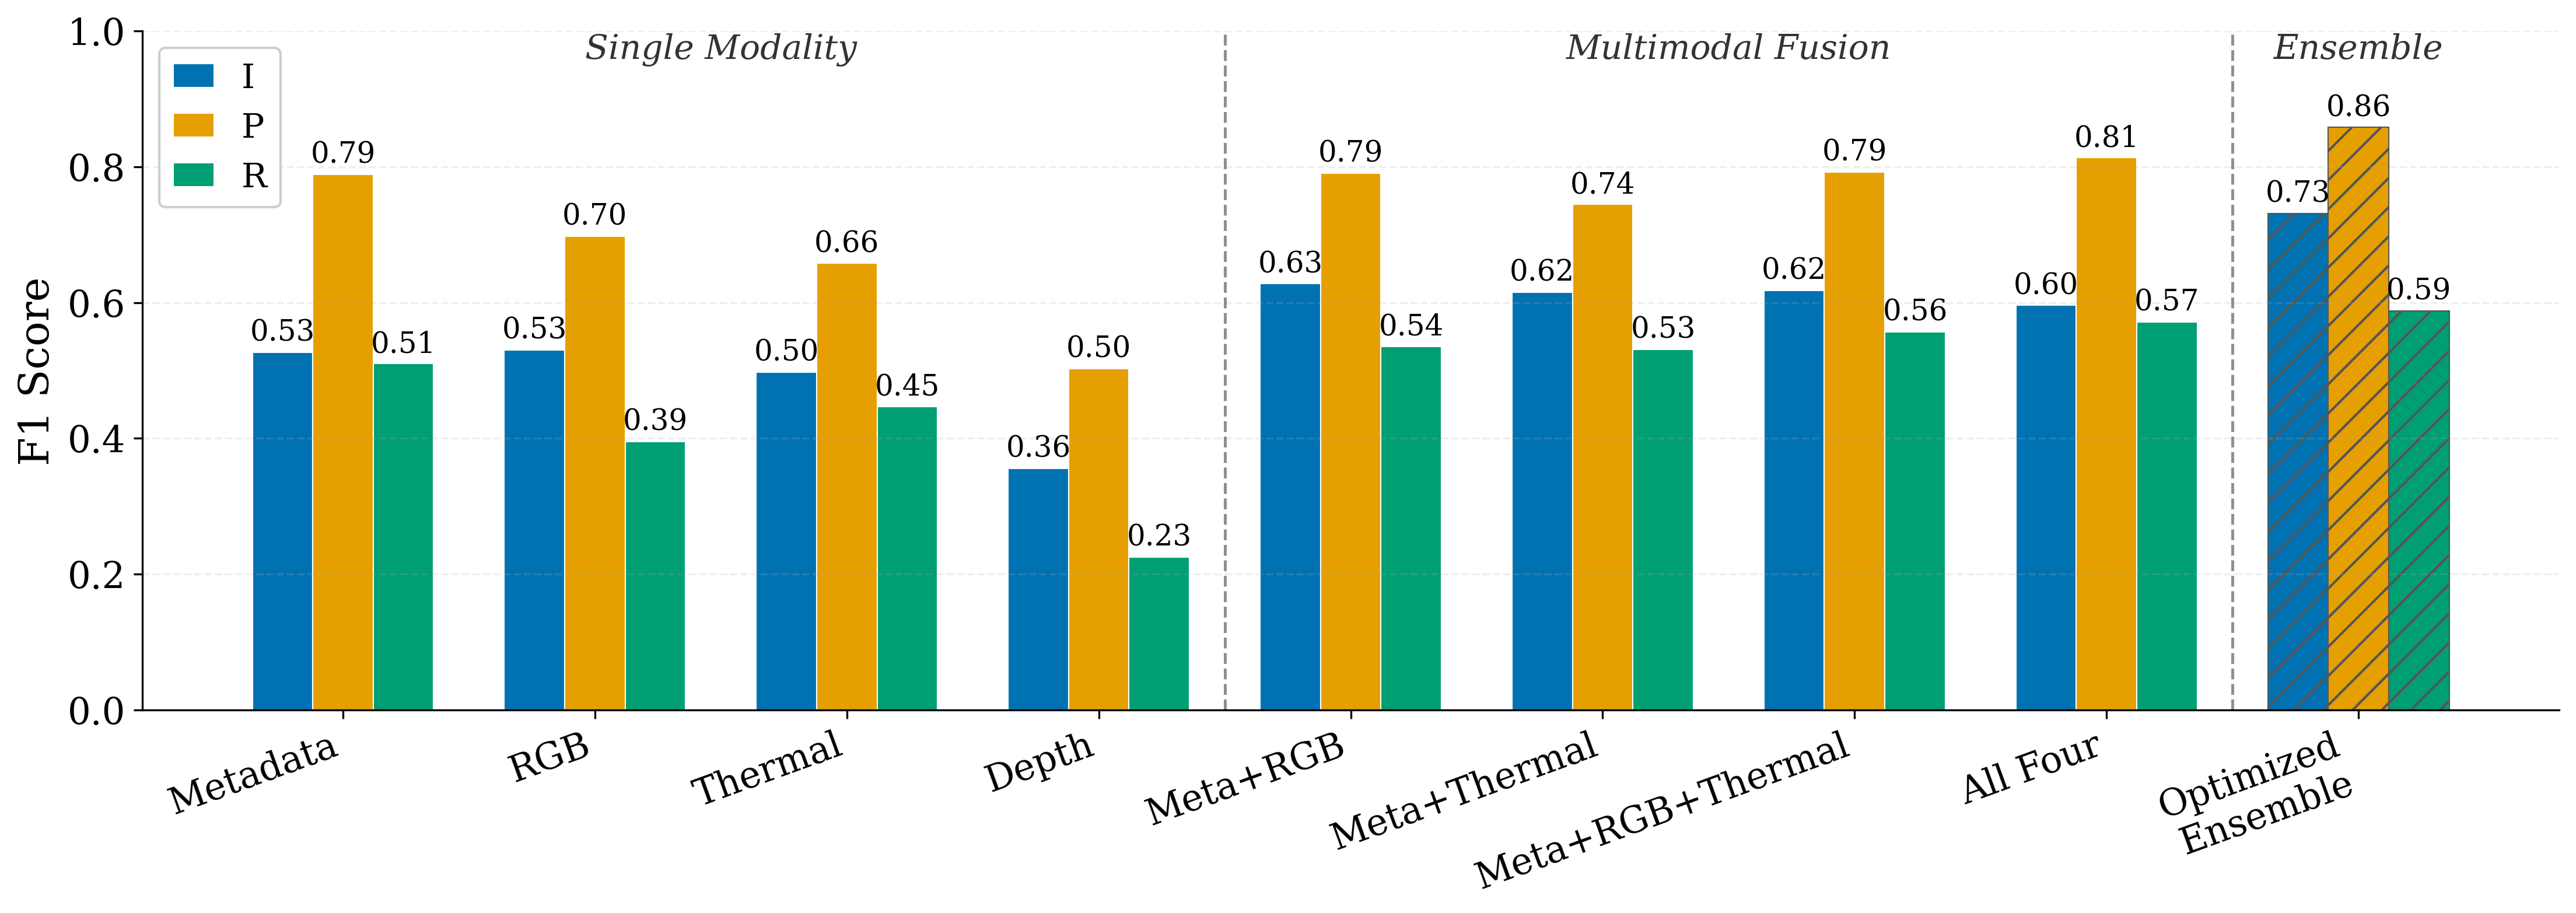
\includegraphics[width=\textwidth]{figures/phase_f1_scores.png}}
\caption{Phase\nobreakdash-Specific F1\nobreakdash-Scores Across Modality Combinations. Comparative analysis highlighting relative performance of various fusion strategies across healing phases in five\nobreakdash-fold cross\nobreakdash-validation.}
\label{fig:phase_f1}
\end{figure*}

Multimodal fusion demonstrated consistent improvements with increasing modality count. Dual modalities improved mean accuracy by 7.6 percentage points over single\nobreakdash-modality baselines (59.2\% to 66.8\%). Triple modalities increased accuracy by an additional 4.2 percentage points (71.0\%), while quaternary fusion achieved 72.0\% accuracy. Cohen's kappa followed the same trend: single 0.43, dual 0.54, triple 0.58, quaternary 0.61.
One\nobreakdash-way ANOVA confirmed significant performance differences across modality group sizes ($F = 5.56$, $p = 0.002$). Linear regression revealed a positive relationship between modality count and kappa (slope $= 0.07$, $R^2 = 0.40$, $p = 0.01$), indicating that each additional modality contributes approximately 0.07 kappa units. McNemar's test confirmed that the best fusion significantly outperformed metadata alone at the sample level ($\chi^2 = 4.56$, $p = 0.03$) and depth alone ($\chi^2 = 84.50$, $p < 0.001$).

The best individual modality combination, metadata + RGB + thermal, achieved Cohen's kappa of 0.61~$\pm$~0.09 and accuracy of 71.24\%. Notably, the top four combinations (all including metadata and RGB) were within 0.01 kappa of each other, indicating that the core metadata + RGB signal accounts for most discriminative power, with thermal and depth providing marginal additional gains.

Figure~\ref{fig:performance_progression} illustrates performance improvement with modality integration, showing incremental gains as additional modalities are incorporated into the fusion framework.

\begin{figure}[!t]
% DONE: Figure generated by paper/generate_figures.py
\centerline{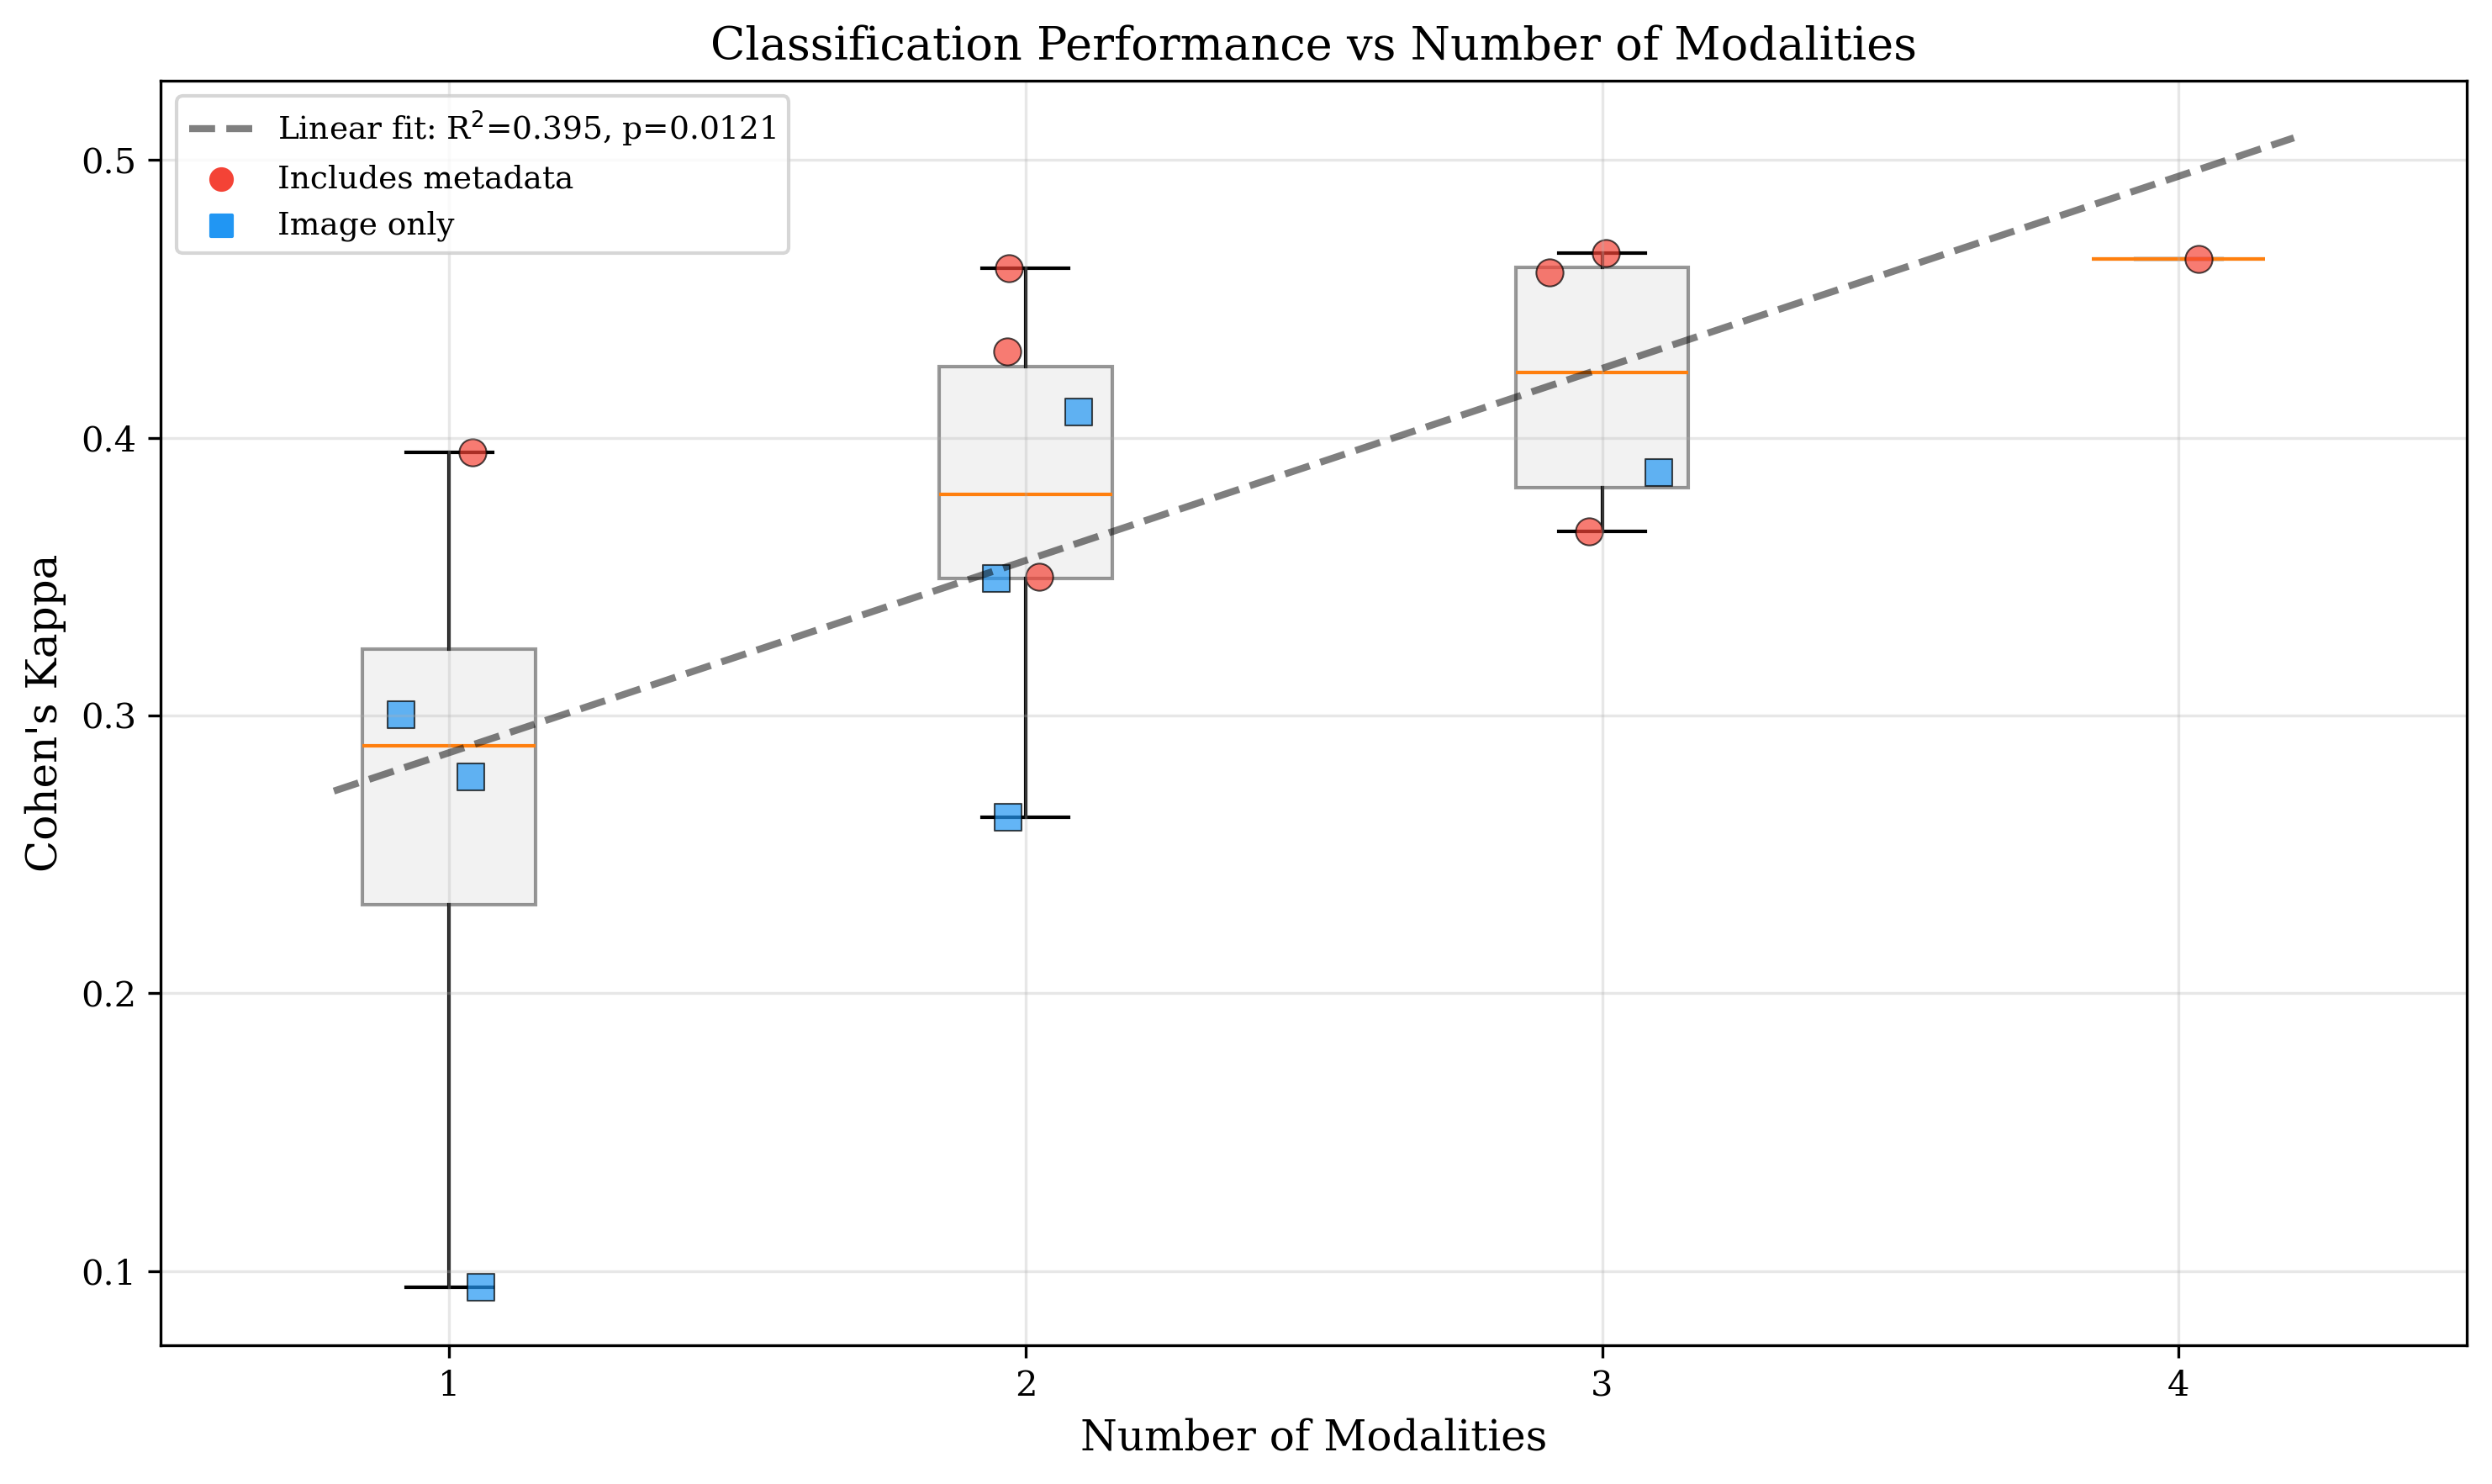
\includegraphics[width=\columnwidth]{figures/performance_progression.png}}
\caption{Performance Progression with Modality Integration. Analysis showing incremental gains in Cohen's kappa as additional modalities integrate into the fusion framework across five\nobreakdash-fold cross\nobreakdash-validation.}
\label{fig:performance_progression}
\end{figure}

\subsection{Modality Contribution Analysis}
Analysis of standalone versus fusion performance revealed the relative contribution of each modality to the combined classification. Metadata consistently served as the strongest individual signal (kappa 0.45), while RGB provided the most complementary imaging information (kappa 0.51). Every fusion combination that included metadata outperformed metadata alone, confirming that image modalities provide additive discriminative value despite their lower standalone performance. Depth maps showed the weakest contribution (kappa 0.19 alone), degrading some combinations they joined. This finding is supported by the raw image analysis: depth maps encode wound surface topology as viridis colormapped distance values, producing low color diversity (median 78 unique colors per crop) with minimal inter-phase variation. Wound surface geometry does not appear to differ systematically across healing phases, whereas wound color (RGB), temperature (thermal), and clinical history (metadata) each capture distinct phase-discriminative characteristics.

Figure~\ref{fig:modality_agreement} visualizes agreement patterns across the three primary modalities (metadata, RGB, thermal), showing the fraction of samples correctly classified by each subset of modalities. This complementarity analysis informed the ensemble design by identifying metadata as the essential anchor modality.

\begin{figure}[!t]
% DONE: Figure generated by paper/generate_figures.py
\centerline{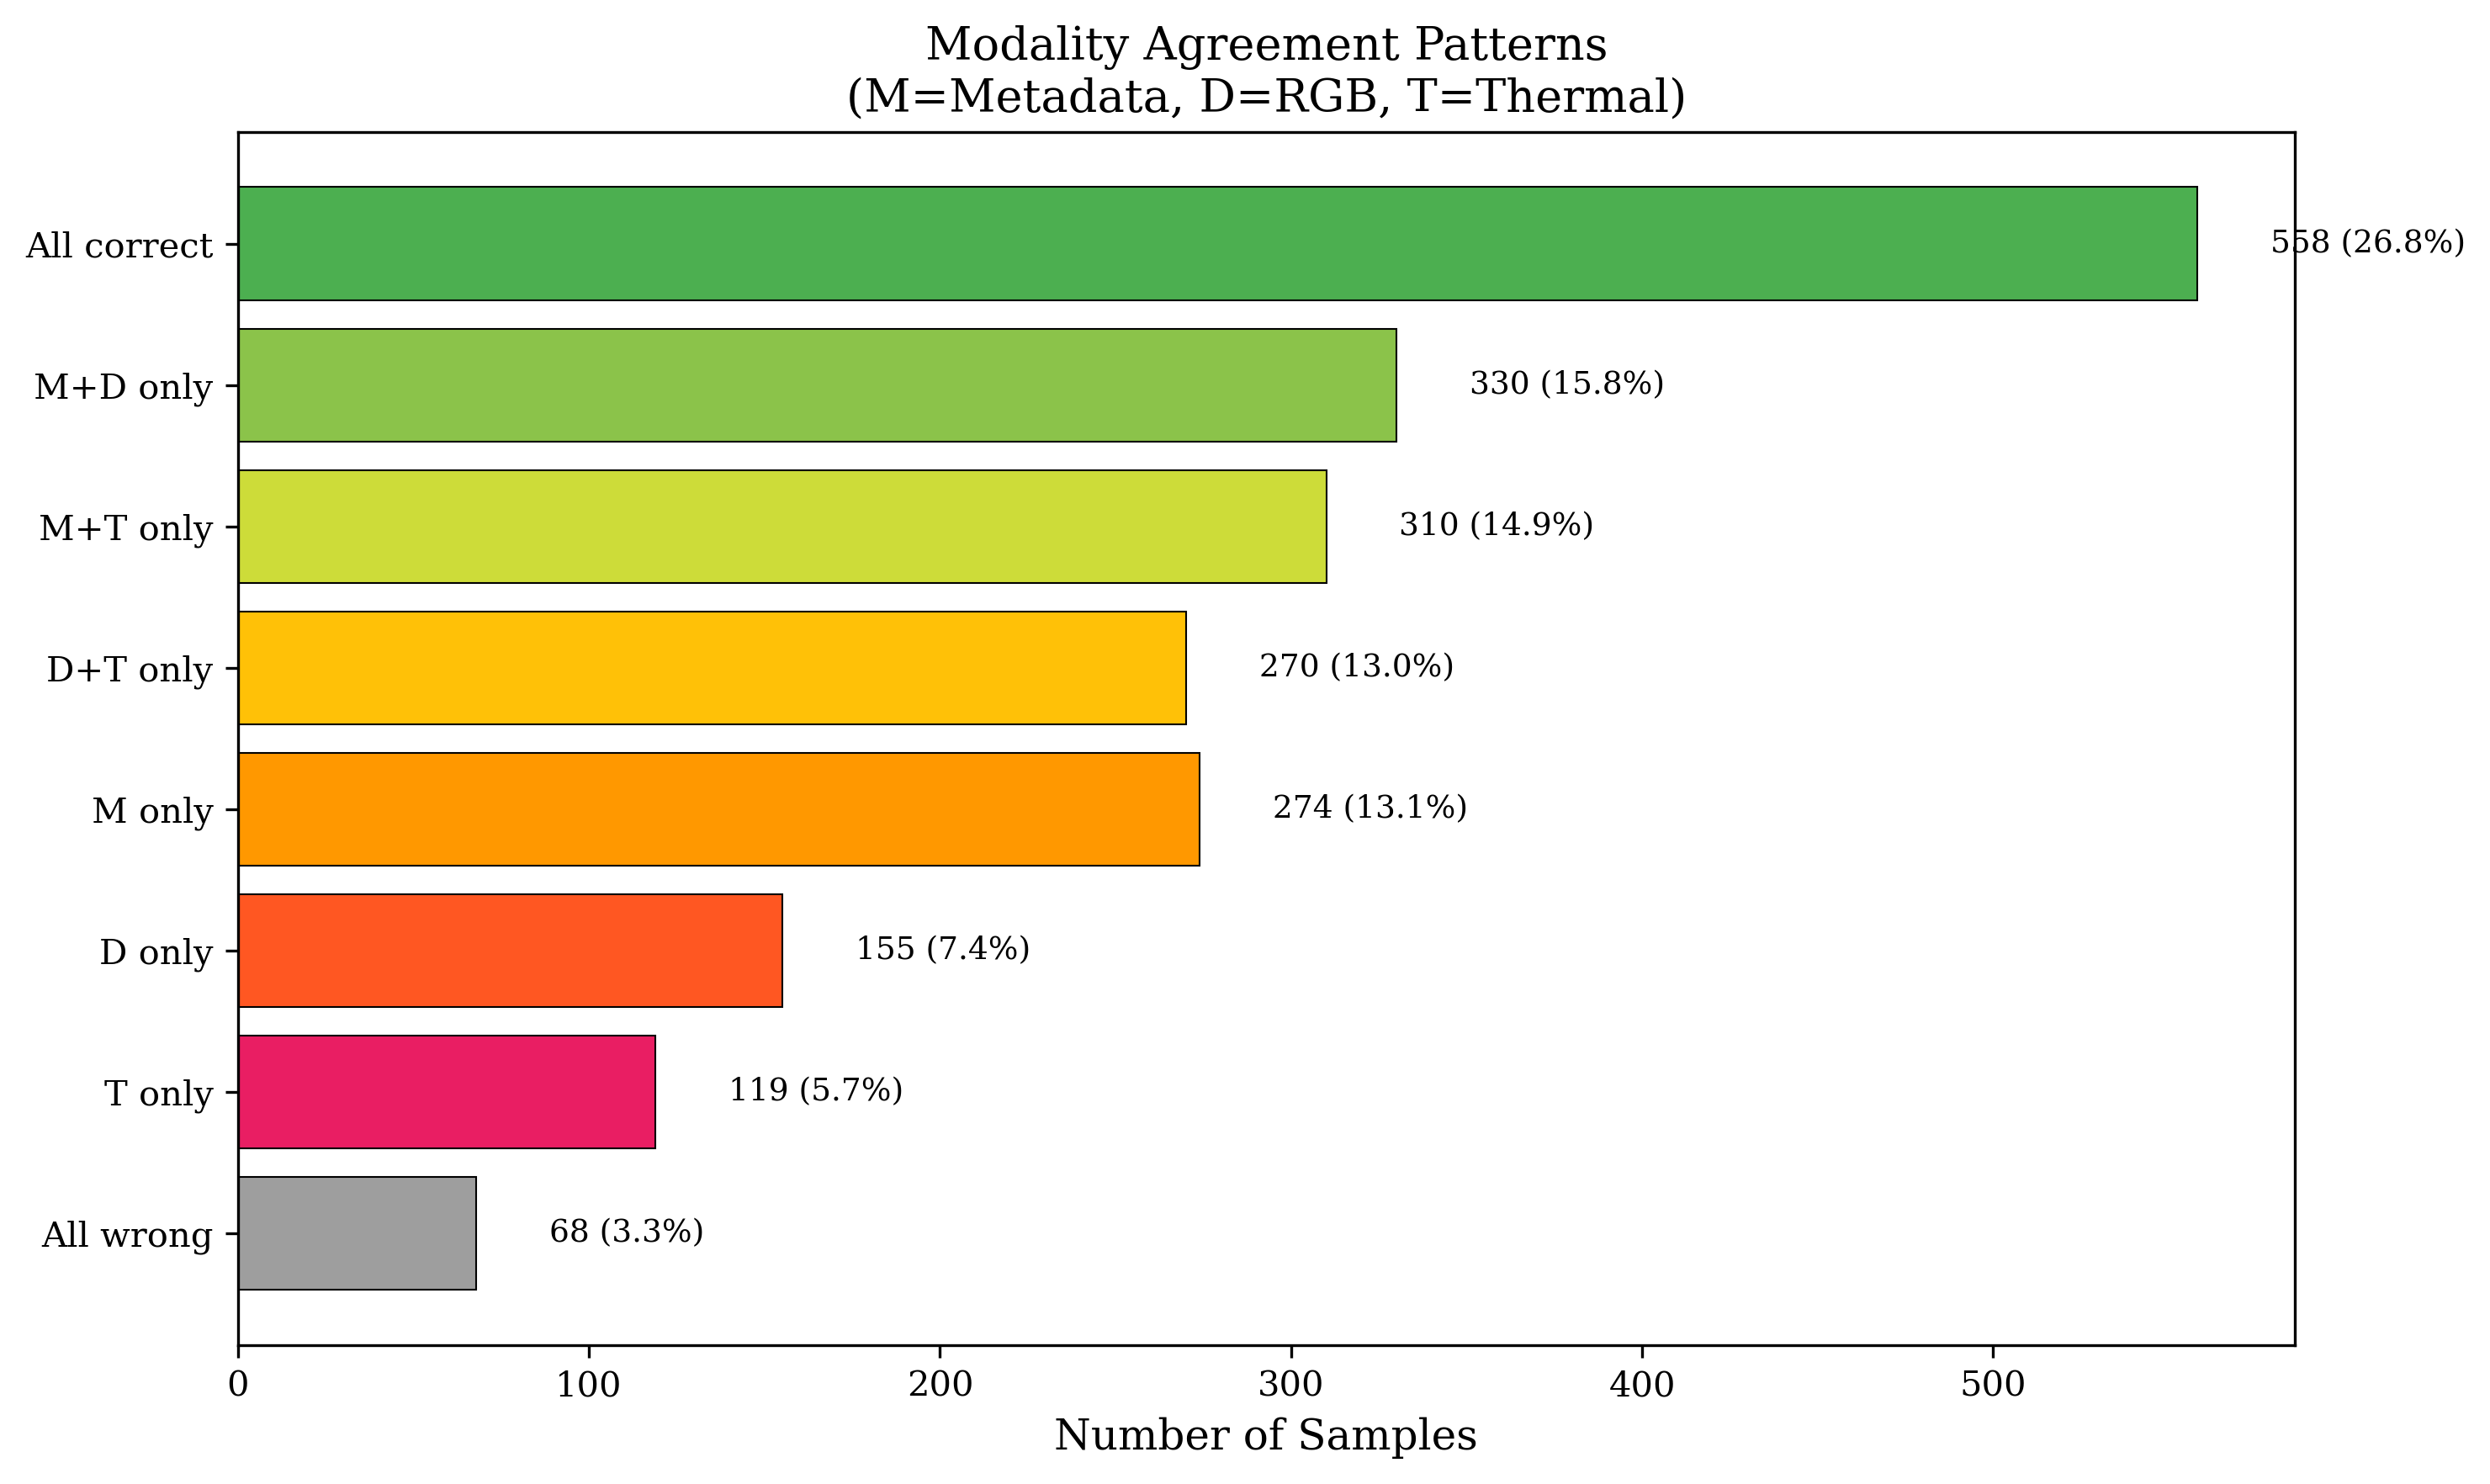
\includegraphics[width=\columnwidth]{figures/modality_agreement.png}}
\caption{Modality Agreement Patterns. Distribution of sample\nobreakdash-level correctness across metadata (M), RGB (D), and thermal (T) modalities, showing the fraction of samples correctly classified by each modality subset. The complementarity between metadata and imaging modalities motivates the ensemble design.}
\label{fig:modality_agreement}
\end{figure}

\subsection{Ensemble Framework Results}
The ensemble combines softmax predictions from all modality combinations that include metadata (8 of 15 total combinations). This parameter\nobreakdash-free approach was selected from 111 configurations spanning eight strategies (Section~\ref{sec:ensemble}). Table~\ref{tab:comprehensive_results} presents comprehensive performance analysis across modality combinations, comparing individual combination results with the ensemble.

\begin{table}[!t]
\renewcommand{\arraystretch}{1.3}
\caption{Performance Analysis Across Key Modality Combinations. Complete results for all 15 combinations are provided in Appendix~A, Table~\ref{tab:supplementary_all_combos}.}
\label{tab:comprehensive_results}
\centering
\begin{tabular}{|l|c|c|c|c|c|}
\hline
\textbf{Modality} & \multicolumn{3}{c|}{\textbf{F1 (\%)}} & \textbf{Accuracy} & \textbf{Cohen's} \\
\textbf{Combination} & \textbf{I} & \textbf{P} & \textbf{R} & \textbf{$\pm$std (\%)} & \textbf{$\kappa$ $\pm$std} \\
\hline
\multicolumn{6}{|l|}{\textit{Single modalities}} \\
\hline
Metadata & 53 & 79 & 51 & 71 $\pm$08 & 0.45 $\pm$0.17 \\
RGB & 59 & 66 & 46 & 61 $\pm$05 & 0.51 $\pm$0.07 \\
Thermal & 54 & 62 & 48 & 58 $\pm$06 & 0.50 $\pm$0.10 \\
Depth & 37 & 52 & 22 & 44 $\pm$09 & 0.19 $\pm$0.05 \\
\hline
\multicolumn{6}{|l|}{\textit{Top fusion combinations}} \\
\hline
Meta + RGB + Thermal & 69 & 76 & 54 & 71 $\pm$04 & 0.61 $\pm$0.09 \\
Meta + RGB & 69 & 77 & 54 & 72 $\pm$04 & 0.61 $\pm$0.07 \\
Meta + RGB + Depth & 67 & 81 & 57 & 75 $\pm$02 & 0.61 $\pm$0.07 \\
Meta + Thermal & 67 & 75 & 57 & 70 $\pm$03 & 0.60 $\pm$0.06 \\
All Four & 67 & 77 & 57 & 72 $\pm$05 & 0.61 $\pm$0.09 \\
\hline
\multicolumn{6}{|l|}{\textit{Ensemble}} \\
\hline
\textbf{Full (8 combos)} & \textbf{68} & \textbf{84} & \textbf{60} & \textbf{79 $\pm$04} & \textbf{0.53 $\pm$0.12} \\
\textbf{Optimized (4 combos)} & \textbf{73} & \textbf{86} & \textbf{59} & \textbf{81 $\pm$05} & \textbf{0.58 $\pm$0.14} \\
\hline
\end{tabular}
\end{table}

The full ensemble (averaging all eight metadata\nobreakdash-containing combinations) achieved the highest accuracy (78.50\%) and balanced per\nobreakdash-class performance among all configurations tested. Leave\nobreakdash-one\nobreakdash-out analysis of ensemble composition revealed that not all combinations contribute equally: metadata alone was the strongest contributor (+0.015 kappa when included), while some high\nobreakdash-performing individual combinations (metadata + RGB + thermal) actually degraded ensemble performance ($-$0.016 kappa) due to overconfident predictions. An optimized four\nobreakdash-combination subset (metadata, metadata + depth, metadata + thermal, metadata + RGB + depth) improved ensemble kappa from 0.53 to 0.58 while maintaining accuracy of 80.56\%. This finding indicates that ensemble diversity, not individual combination performance, determines ensemble effectiveness.

Figure~\ref{fig:dose_response} shows the effect of generative augmentation probability on ensemble performance, illustrating the inverted\nobreakdash-U dose\nobreakdash-response with optimal F1\nobreakdash-R at 15\% injection probability.

\begin{figure}[!t]
% DONE: Figure generated by paper/generate_figures.py
\centerline{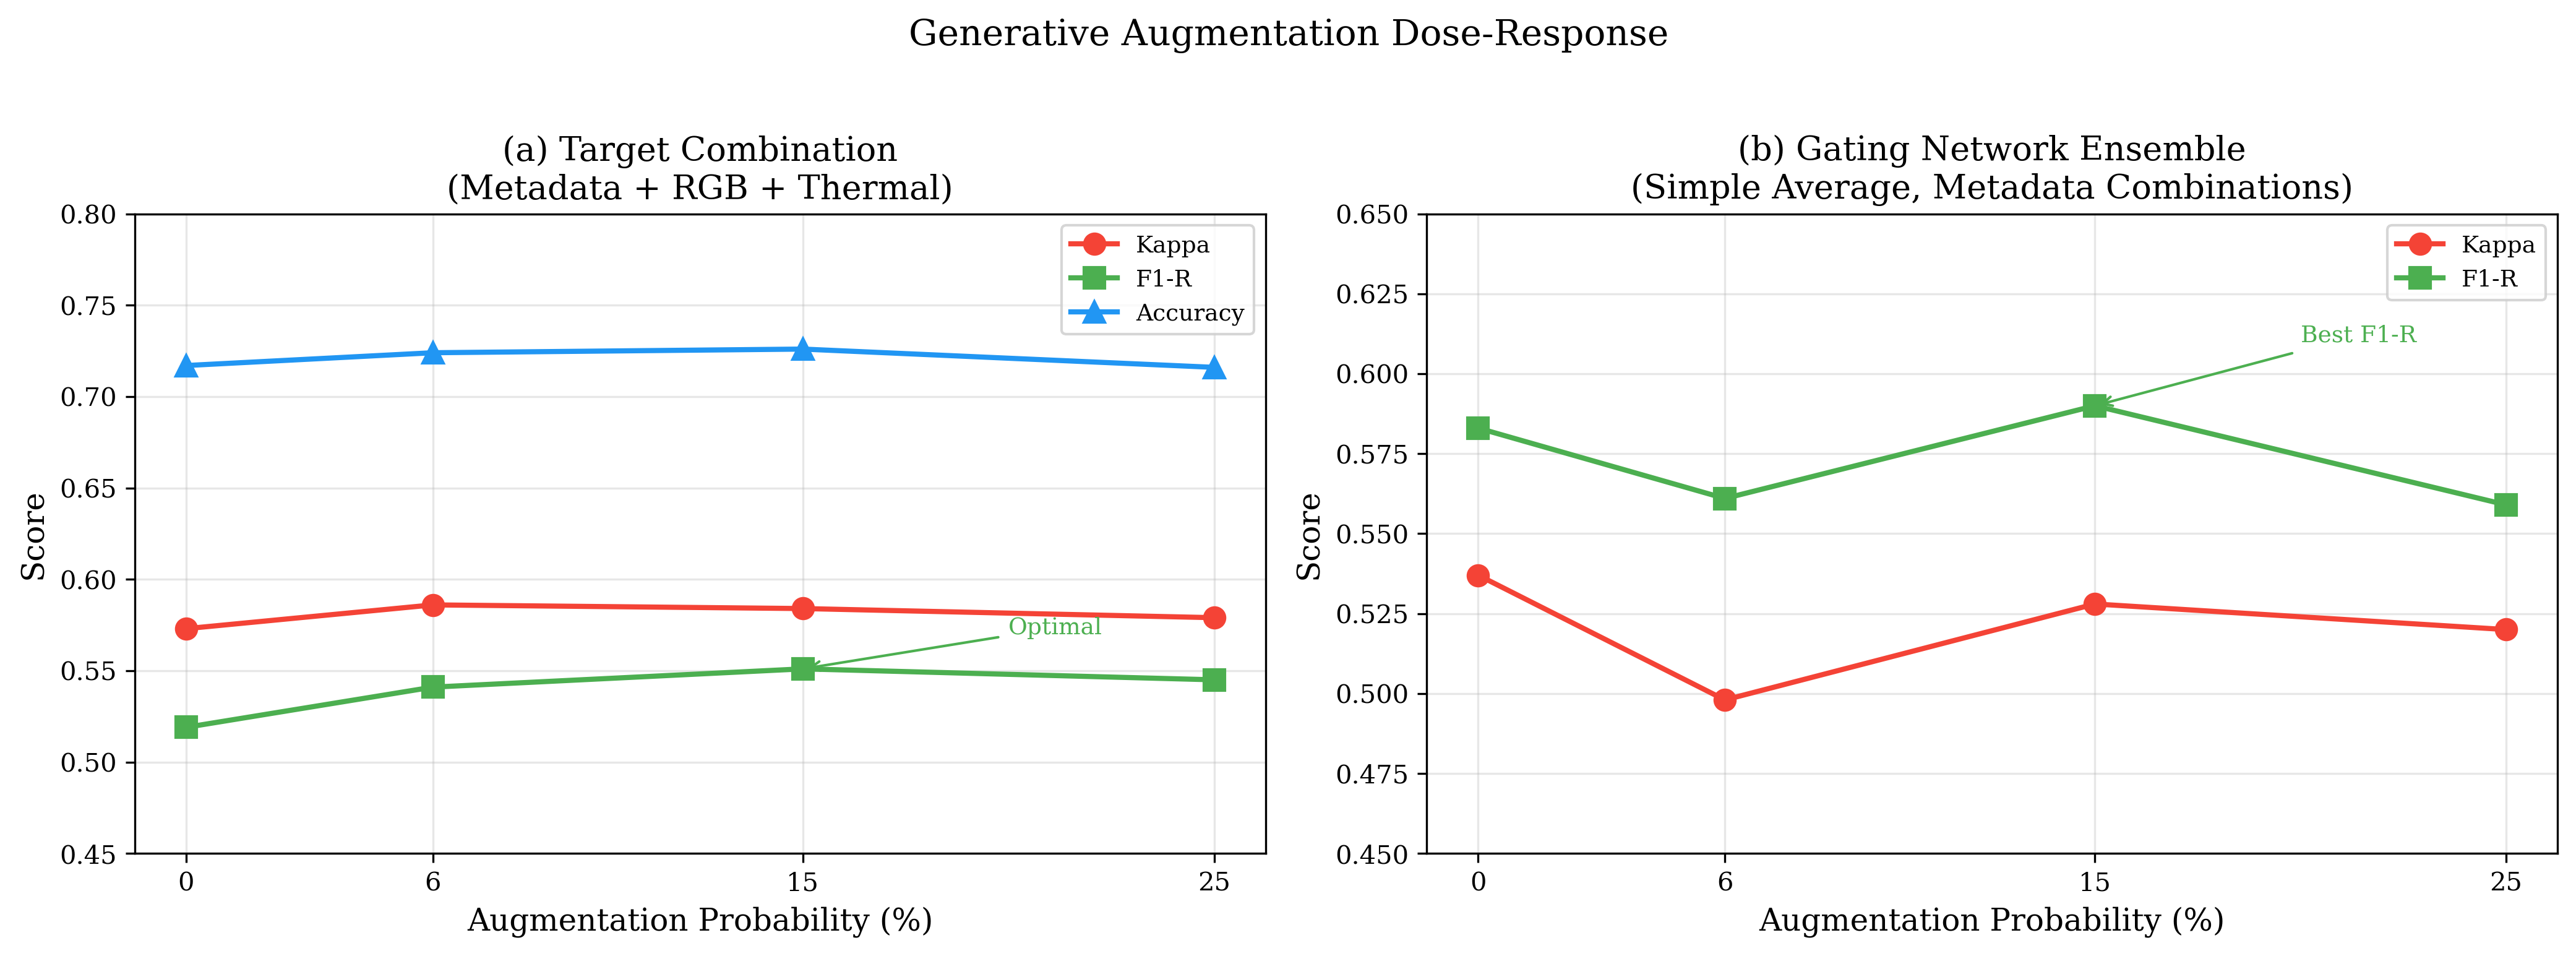
\includegraphics[width=\columnwidth]{figures/dose_response.png}}
\caption{Generative Augmentation Dose\nobreakdash-Response. Effect of augmentation injection probability on the target modality combination (metadata + RGB + thermal, solid lines) and ensemble (dashed lines). F1\nobreakdash-R peaks at 15\% for the ensemble (0.59), while higher probabilities degrade performance due to overfitting to the fixed synthetic image cache.}
\label{fig:dose_response}
\end{figure}

\section{Discussion}

\subsection{Clinical Significance and Innovation}
DFU\nobreakdash-MFNet represents a significant advancement in automated DFU assessment, achieving Cohen's kappa of 0.61 and accuracy of 75.38\% in healing phase classification without laboratory diagnostics. This performance approaches practical clinical decision support requirements while maintaining accessibility across diverse healthcare settings. Multimodal fusion improved mean kappa from 0.43 (single\nobreakdash-modality average) to 0.61 (best fusion combination), demonstrating substantial value of multimodal integration in capturing complex wound healing progression.

The modality contribution analysis revealed a clear implementation hierarchy: metadata provides the strongest standalone signal (kappa 0.45), while RGB imaging offers the most complementary information (every metadata + RGB combination outperforms metadata alone). This hierarchy provides evidence\nobreakdash-based guidance for resource\nobreakdash-adaptive clinical implementation, from basic electronic health record integration to comprehensive multimodal assessment systems. Importantly, thermal mapping contributes to balanced per\nobreakdash-class performance, particularly for the minority remodeling phase (F1\nobreakdash-R: 0.57 for metadata + thermal vs 0.54 for metadata + RGB).

From a clinical perspective, these findings offer insight into which physical characteristics differentiate healing phases. Metadata (patient demographics, wound scores, temperature readings) captures systemic factors that broadly predict healing trajectory, while RGB imaging captures wound surface morphology (color, texture, tissue composition) that distinguishes inflammatory from proliferative phases. Thermal mapping captures subsurface vascular activity that is particularly informative for identifying the remodeling phase, where reduced metabolic activity produces distinct thermal signatures. Depth sensing alone carries minimal phase\nobreakdash-discriminative information (kappa 0.19), suggesting that wound topology is not a reliable indicator of healing phase in isolation. These observations inform both clinical assessment priorities and future sensor development for wound monitoring devices.

Existing clinical classification systems such as the University of Texas, Wagner, and WIfI focus on wound severity, infection risk, and amputation probability, providing essential treatment urgency assessment. DFU\nobreakdash-MFNet complements these systems by adding temporal healing phase characterization, which these classification systems do not address. Where WIfI determines \textit{what} intervention is needed based on current wound state, healing phase classification determines \textit{when} to adjust treatment based on the biological stage of tissue repair. Integrating both approaches could enable clinicians to combine severity assessment with phase-aware treatment selection, for example adjusting growth factor therapies during the proliferative phase or identifying stalled inflammatory responses that require intervention.

\subsection{Comparison with Existing Approaches}
Direct comparison reveals novel contributions versus existing systems. While Al\nobreakdash-Garaawi et al.~\cite{al2022diabetic} reported F1\nobreakdash-scores of 0.95\nobreakdash-0.99 for binary RGB\nobreakdash-thermal classification, and Reyes\nobreakdash-Lu\'{e}vano et al.~\cite{reyes2023dfu} achieved 0.96 for binary classification, these approaches do not address temporal healing complexity. Our three\nobreakdash-class healing phase discrimination provides substantially higher clinical value, directly informing phase\nobreakdash-specific therapeutic interventions.

The jointly optimized fusion framework achieved Cohen's kappa of 0.61 with ensemble accuracy of 78.86\%, representing a novel contribution to multimodal fusion strategies for medical imaging. A key finding is that feature concatenation fusion with jointly optimized components outperforms more complex attention\nobreakdash-based approaches when training data is limited (443 samples). This aligns with established machine learning principles favoring simpler models under data constraints~\cite{kebaili2023deep}.

\subsection{Joint Optimization and Architectural Insights}
The joint Bayesian optimization revealed several findings that contradict conventional assumptions in medical image analysis. First, DenseNet121~\cite{huang2017densely} outperformed EfficientNet~\cite{tan2019efficientnet} for both RGB and thermal modalities, despite EfficientNet's widespread adoption in medical imaging. DenseNet's dense connectivity and feature reuse may provide superior transfer learning for false\nobreakdash-color medical images that differ substantially from ImageNet's natural image domain. Second, reducing input resolution from 256$\times$256 to 128$\times$128 pixels improved performance, because the average wound bounding box is only 70$\times$70 pixels; at 256$\times$256, the 3\nobreakdash-14$\times$ upsampling introduces interpolation artifacts that obscure genuine wound texture. Third, simple probability averaging of metadata\nobreakdash-containing combinations outperformed all 111 tested ensemble strategies including multi\nobreakdash-head attention, MLP stacking, and gradient boosting. The attention\nobreakdash-based gating network collapsed to majority\nobreakdash-class prediction on two of five folds, confirming that complex ensemble architectures are prone to overfitting with limited training data.

\subsection{Generative Augmentation and Technical Innovation}
Implementation of SDXL\nobreakdash-based generative augmentation addresses the fundamental challenge of class imbalance in medical datasets. The dose\nobreakdash-response characterization across three injection probabilities (6\%, 15\%, 25\%) revealed an inverted\nobreakdash-U relationship: F1\nobreakdash-R for the minority remodeling class improved from 0.52 (no augmentation) to 0.55 (15\%), then declined at 25\% due to overfitting to the fixed synthetic image cache. This finding provides practical guidance for calibrating augmentation intensity, which has received limited systematic investigation in medical imaging~\cite{kebaili2023deep}. FID scores confirmed preservation of phase\nobreakdash-specific characteristics in the generated images.

This work represents among the first applications of SDXL\nobreakdash-based synthetic image generation specifically for DFU wound classification. The pre\nobreakdash-caching approach (generating synthetic images to disk before training) provides a practical solution for dual\nobreakdash-framework environments where PyTorch\nobreakdash-based generation and TensorFlow\nobreakdash-based training cannot share GPU memory. The decision to limit augmentation to RGB imagery reflects important considerations regarding the measurement\nobreakdash-based nature of thermal and depth modalities.

\subsection{Resource Adaptation and Implementation}
DFU\nobreakdash-MFNet's modular architecture enables effective implementation across diverse healthcare settings. In our previous work~\cite{basiri2021reduction}, we demonstrated that a metadata\nobreakdash-driven approach, utilizing a larger dataset, achieves 69\% accuracy and provides fundamental triage capabilities. In the present study, requiring all four modalities for each sample reduces the available dataset size, yet metadata alone still achieves 70.55\% accuracy. Following the observed increasing performance trend with additional modalities, the integration of RGB imaging with metadata should be prioritized (kappa improvement from 0.45 to 0.61), followed by thermal imaging for improved minority class performance. Sites supporting all four modalities can implement the full DFU\nobreakdash-MFNet architecture with ensemble framework, achieving the highest overall accuracy (78.86\%).

\subsection{Limitations and Future Directions}
Several limitations warrant acknowledgment. Class imbalance (I:~23\%, P:~63\%, R:~13\%), while reflecting clinical reality, presents analytical challenges particularly for the remodeling phase (58 samples after screening), potentially affecting generalizability. The single\nobreakdash-site dataset may not capture demographic diversity across healthcare systems, requiring multi\nobreakdash-institutional validation.

Imaging equipment requirements (approximately \$3,000\nobreakdash-\$5,000 per unit) may represent barriers for primary care adoption, though costs are reasonable for specialized wound care centers. Each image preprocessing step isolated single wound areas, limiting capability for simultaneous multiple ulceration analysis present in complex clinical scenarios. The generative augmentation cache size (144 images per phase) constrains the maximum useful injection probability; larger caches may extend the useful augmentation range.

Future directions include longitudinal validation studies enabling healing trajectory prediction, multi\nobreakdash-site validation across diverse clinical settings, and clinician\nobreakdash-in\nobreakdash-the\nobreakdash-loop studies evaluating optimal human\nobreakdash-artificial intelligence collaboration strategies. Technical advances could include domain\nobreakdash-specific pretraining on wound image corpora, expanded generative caches with diversity\nobreakdash-aware sampling, and physics\nobreakdash-informed generative models preserving measurement characteristics across modalities.

\section{Conclusion}
This paper introduces DFU\nobreakdash-MFNet, a multimodal fusion network addressing critical gaps in DFU healing phase classification. Through systematic investigation of fusion strategies, joint Bayesian optimization, and ensemble methods, this work establishes quantitative evidence for the complementary value of integrating clinical metadata, RGB imaging, thermal mapping, and depth sensing in wound evaluation.

Key contributions include: the DFU\nobreakdash-MFNet architecture with jointly optimized feature concatenation fusion achieving Cohen's kappa of 0.61 and accuracy of 75.38\% in three\nobreakdash-class healing phase classification; demonstration that joint optimization of all pipeline components outperforms sequential per\nobreakdash-modality tuning (kappa improved from 0.30 to 0.61); characterization of SDXL\nobreakdash-based generative augmentation dose\nobreakdash-response with optimal minority class recall improvement of 0.03 at 15\% injection probability; and a parameter\nobreakdash-free ensemble framework achieving 78.86\% accuracy by averaging predictions from metadata\nobreakdash-containing modality combinations.

Experimental validation on 443 wound assessments from 233 patients using five\nobreakdash-fold patient\nobreakdash-stratified cross\nobreakdash-validation demonstrates framework effectiveness across diverse clinical presentations. Statistical analyses confirmed significant performance improvements across modality combinations ($p < 0.05$).
% DONE: p-values computed — McNemar's test: fusion vs metadata p=0.03*, fusion vs depth_rgb p<0.001***. Paired t-test: fusion vs metadata p=0.34 (ns on fold-level kappa, significant at sample level via McNemar's). See paper/statistics/

Clinical significance lies in the potential to enhance treatment planning through accurate phase identification while maintaining adaptability across healthcare settings. The modular architecture supports resource\nobreakdash-adaptive deployment from basic metadata\nobreakdash-only triage (kappa 0.45) to comprehensive multimodal assessment (kappa 0.61), enabling objective wound evaluation supporting phase\nobreakdash-specific therapeutic interventions without laboratory diagnostics.

\section*{Data and Code Availability}
The code used in this study is publicly available through the GitHub repository "DFUMultiClassification" at \url{https://github.com/rezabasiri/DFUMultiClassification}. The resulted model weights are also provided in this repository for deployment and evaluation on publicly available single modality datasets such as DFU2020 \cite{yap2021deep} or Plantar Thermogram Database \cite{hernandez2019plantar}. The four-modality training dataset cannot be shared publicly at this point because the release of data was not included in the ethics approval. While it is beneficial to enable public access to the Zivot dataset for additional validations and research, the modality analyses and provision of the DFU\nobreakdash-MFNet method with a detailed description of features collected from patients presented in previous works~\cite{basiri2024accessible,basiri2024protocol} stands as an independent contribution. We are actively working towards public dataset availability, navigating through challenges and dedicating substantial time and resources to make this possible. We plan to facilitate the release of the dataset to selected research institutes upon request after ethics amendment approvals.

\section*{Acknowledgment}
The authors thank the clinicians and staff at the Zivot Limb Preservation Centre for their invaluable support in data collection and clinical expertise. We acknowledge the patients who participated in this study and the technical support provided by the research teams at the University of Toronto, University Health Network and Alberta Health Services.

\bibliographystyle{IEEEtran}
\bibliography{references}
\vspace{-1.3cm}
\begin{IEEEbiography}[{\includegraphics[width=1in,height=1.25in,clip,keepaspectratio]{author1.jpg}}]{Reza Basiri}
(Student Member, IEEE) received the B.Sc. degree in biomedical engineering from the University of Calgary, Calgary, AB, Canada, in 2019, and is currently pursuing the Ph.D. degree with the Institute of Biomedical Engineering, University of Toronto, Toronto, ON, Canada. His research interests include medical image analysis, multimodal machine learning, and artificial intelligence applications in wound care and diabetic foot ulcer management.
\end{IEEEbiography}
\vspace{-1.55cm}
\begin{IEEEbiography}[{\includegraphics[width=1in,height=1.25in,clip,keepaspectratio]{author2.jpg}}]{Milos R. Popovic}
(Fellow, IEEE) received the Ph.D. degree in electrical engineering from McGill University, Montreal, QC, Canada, in 1993. He is currently a Professor and the Director of the Institute of Biomedical Engineering, University of Toronto, Toronto, ON, Canada, and Director of The KITE Research Institute. His research interests include functional electrical stimulation, neural engineering, and rehabilitation technologies. He has authored over 200 peer-reviewed publications and holds several patents in biomedical engineering.
\end{IEEEbiography}
\vspace{-1.55cm}
\begin{IEEEbiography}[{\includegraphics[width=1in,height=1.25in,clip,keepaspectratio]{author3.jpg}}]{Shehroz S. Khan}
(Senior Member, IEEE) received the Ph.D. degree in computer science from the University of Western Ontario, London, ON, Canada, in 2010. He is currently an Associate Professor with the Department of Electrical Engineering and Computer Science, York University, Toronto, ON, Canada, and a Scientist with KITE – Toronto Rehabilitation Institute, University Health Network. His research interests include machine learning, artificial intelligence, and data mining with applications in healthcare and cybersecurity.
\end{IEEEbiography}

\newpage
\appendices
\section{Complete Modality Combination Results}
\label{app:all_combos}

\begin{table*}[H]
\renewcommand{\arraystretch}{1.2}
\caption{Complete Performance Analysis for All 15 Modality Combinations (five-fold patient-stratified cross-validation with 15\% generative augmentation)}
\label{tab:supplementary_all_combos}
\centering
\begin{tabular}{|l|c|c|c|c|c|c|c|}
\hline
\textbf{Modality Combination} & \textbf{F1-I} & \textbf{F1-P} & \textbf{F1-R} & \textbf{Acc (\%)} & \textbf{$\pm$std} & \textbf{$\kappa$} & \textbf{$\pm$std} \\
\hline
\multicolumn{8}{|l|}{\textit{Single modalities}} \\
\hline
Metadata & 0.53 & 0.79 & 0.51 & 70.55 & 8.42 & 0.45 & 0.17 \\
RGB & 0.59 & 0.66 & 0.46 & 60.96 & 4.73 & 0.51 & 0.07 \\
Thermal & 0.54 & 0.62 & 0.48 & 58.13 & 5.94 & 0.50 & 0.10 \\
Depth & 0.37 & 0.52 & 0.22 & 44.21 & 9.22 & 0.19 & 0.05 \\
\hline
\multicolumn{8}{|l|}{\textit{Dual modalities}} \\
\hline
Metadata + RGB & 0.69 & 0.77 & 0.54 & 72.28 & 3.61 & 0.61 & 0.07 \\
Metadata + Thermal & 0.67 & 0.75 & 0.57 & 70.20 & 3.42 & 0.60 & 0.06 \\
Metadata + Depth & 0.54 & 0.74 & 0.44 & 66.54 & 10.45 & 0.44 & 0.10 \\
RGB + Thermal & 0.59 & 0.76 & 0.50 & 70.05 & 12.79 & 0.55 & 0.13 \\
RGB + Depth & 0.52 & 0.74 & 0.45 & 67.04 & 8.65 & 0.47 & 0.10 \\
Depth + Thermal & 0.49 & 0.64 & 0.44 & 58.34 & 7.21 & 0.45 & 0.11 \\
\hline
\multicolumn{8}{|l|}{\textit{Triple modalities}} \\
\hline
Meta + RGB + Thermal & 0.69 & 0.76 & 0.54 & 71.24 & 4.49 & 0.61 & 0.09 \\
Meta + RGB + Depth & 0.62 & 0.81 & 0.53 & 73.59 & 10.89 & 0.57 & 0.11 \\
Meta + Depth + Thermal & 0.55 & 0.70 & 0.47 & 63.53 & 11.26 & 0.50 & 0.11 \\
RGB + Depth + Thermal & 0.56 & 0.74 & 0.48 & 67.66 & 12.11 & 0.52 & 0.12 \\
\hline
\multicolumn{8}{|l|}{\textit{Quaternary}} \\
\hline
All Four Modalities & 0.67 & 0.77 & 0.57 & 71.95 & 4.99 & 0.61 & 0.09 \\
\hline
\end{tabular}
\end{table*}

\end{document}